\newpage
\section{The Quantum Integer Multiplier}

In this section we are going to implement a quantum circuit that computes the product
of two 2-qubit numbers. We are going to first discuss the design of the classic circuit
and then focus on the implementation of its quantum analogue using the Qiskit SDK.

\subsection{Analysing the diagram and logic of the classical Integer Multiplier circuit}

The Integer Multiplier circuit, or just the Multiplier circuit, is a digital circuit that
takes two $n$-bit inputs and computes their arithmetic product. The circuit we are going to
analyse implements the binary multiplication algorithm, by first computing the partial products
and then summing them up to produce the final product \cite{ManoCiletti2018}.

Let $A$ and $B$ be two $n$-bit classic registers. For the purposes of simplicity let $n = 2$.
To compute their multiplication product we first produce the \textit{partial products} of $A \times B$.
This is done digitally by applying an AND gate on every $A_i$ and $B_j$ pair. Then we apply a Half-Adder
for the partial products. We note that the LSB of $PP$ does not need to be added to the Half-Adders.

\begin{table}[ht]
    \centering
    \begin{tabular}{ccccc}
        $$ & $$ & $$ & $B_1$ & $B_0$ \\
        $$ & $$ & $+$ & $A_1$ & $A_0$ \\
        $$ & \cline{2-4}
        $$ & $$ & $$ & $PP_1$ & $PP_0$ \\
        $$ & $\times$ & $PP_3$ & $PP_2$ & $$ \\
        \hline
        $$ & $P_3$ & $P_2$ & $P_1$ & $P_0$ \\
    \end{tabular}
    \caption{Multiplication for two 2-bit integers}
\end{table}

\begin{figure}[ht]
    \centering
    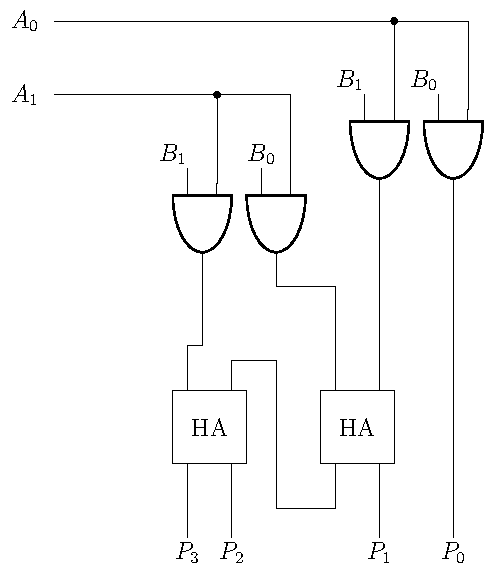
\includegraphics[height=6cm]{images/5_Implementation/classical_2bit_multiplier.pdf}
    \caption{The diagram of the classical Multiplier circuit for two 2-bit inputs}
\end{figure}

\subsection{The Python3 implementation}

The quantum implementation is an expensive circuit, qubit-wise, as it needs to compute the
partial products. As we mentioned previously, the AND function can be simulated by the Toffoli gate
by using one \say{garbage} qubit to store the conjunction of the two conrtol qubits, thus we
need $n^2$ qubits to store the partial products of two $n$-qubit inputs.

As always we initialize the circuit with the two 2-qubit input registers $A$ and $B$. We also
include in our circuit the $2n^2$-qubit auxillary quantum register.

\begin{listing}[ht]
    \centering
    \begin{minted}{python3}
        from qiskit import QuantumCircuit, QuantumRegister

        n = 2
        a = QuantumRegister(n, name="A")
        b = QuantumRegister(n, name="B")
        aux = QuantumRegister(2*n**2, name="aux")

        circuit = QuantumCircuit(a, b, aux)
    \end{minted}
    \caption{Initialization of the quantum Multiplier circuit}
\end{listing}

We proceed to compute the partial-products of $A \times B$ by applying the CNOT gate for each
qubit-pair $A_iB_j$.

\begin{listing}[ht]
    \centering
    \begin{minted}{python3}
        k = 0
        for i in range(n):
            for j in range(n):
                circuit.cx(a[i], b[j], aux[k])
                k += 1
    \end{minted}
    \caption{Computing the partial-products for the quantum Multiplier circuit}
\end{listing}

Despite the expensive nature of the circuit, the overall compexity is pretty low due to the modular
nature of the circuit. We can use the $QFA$ from Section 5.2 to implement the additions of the partial products
but we have to be careful as to which pair of inputs we supply the $QFA$s.

\begin{listing}[ht]
    \centering
    \begin{minted}{python3}
        circuit.append(qfa, (aux[1], aux[2], aux[4], aux[5]))
        circuit.append(qfa, (aux[3], aux[5], aux[6], aux[7]))
    \end{minted}
    \caption{Summing the partial-products to compute the product of $A\times B$}
\end{listing}

To produce the products we need to compute the sum of $P_1+P_2$. This in-turn will produce a sum and a carry-out,
$P_1$ and $C_{out_0}$. The $C_{out_0}$ will be used for the next addition with $P_3$. Finally, after the last
addition we have computed the product of $A \times B$. The output is stored in qubits $P_0$, $Out_0$, $Out_2$ and $Out_3$,
with $Out_2$ be the most-significant qubit of the product.

\begin{figure}[ht]
    \centering
    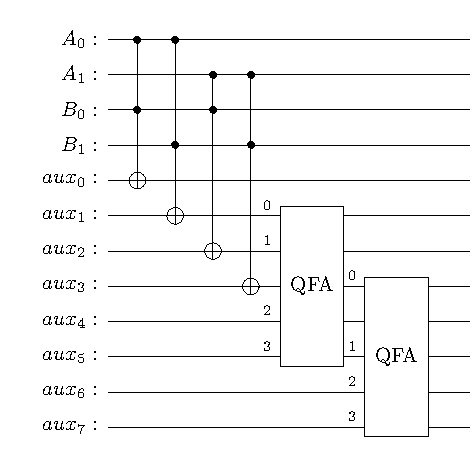
\includegraphics{images/5_Implementation/quantum_2bit_multiplier_with_qfa.pdf}
    \caption{The complete quantum Multiplier unit for 2-qubit inputs}
\end{figure}